\subsection{The Nature of Entrepreneurial Process}
\label{sec:gote}
Jeoroen Kraaijenbrink has made a paper on the entrepreneurial process \cite{kraaijenbrink}. The focuses on the dimensions of the different models rather than the models themselves, as well as a suggestion on connection the nature of entrepreneurship with the nature of human actions. The connection to the human actions is mostly a suggestions, with a few relations to how the human actions are biased. We will talk about our idea in relation to the dimensions mentioned in the paper. Furthermore, We bring a suggestion to an extended version of this model, combining the model with a cognitive process.

\subsubsection*{Dimensions}
As the paper suggests, the process can be tailored in many different ways, as there is no single correct process. Our project is based on an idea, and how this idea can be brought to life. On first glance, this is a ends-driven process, but it can easily be tailored as a means-driven process. This would cause the means to be of more value than the goal, and the goal is open for change. What cause is taken is based on whether we have an affection to Watchr as a service, or it is the entrepreneurial process and the final expectations that have focus.

The most certain of the dimensions for this project is the fact that it focuses on cooperation with existing companies. If we only compete with the market, we will have no suppliers.

The service we are creating is focused on an existing market. The service itself is new, yet its content is already existing. Netflix is the closest to an existing service with the same capabilities, and we try to take this idea even further. To this extend, we are creating an existing service to an existing market, but it can be argued that the service itself is new.

If we try to predict the outcome of the service in hope of controlling the process, we should focus on the existing market. The users should be found to some extend, and whether these are willing to pay for our service. On the other hand, if we control in order to avoid the need to predict, we should focus on previous models for existing and thriving services. Although we can be seen as a new service, we are in an existing market, which makes it possible to gain a certain level of control.

It is a fact that the service is most successful if we have all streaming services available. But the cost for obtaining this level of service, it comes at a great cost. The question is whether we are able to walk away unharmed in case the project fails. The dimension choice of either expecting good results or only commit what we can afford to lose is important, yet hard to make. It is a subjective choice, which depends on the management for the project, and the likeliness of success.

\subsubsection*{GOTE}
G.O.T.E. is an acronym created by Robert Cohen and a method used in theatre and drama \cite{gote}. The method is normally used for reminding the actor of four elements needed when creating a character and its situation. The acronym is for \emph{Goal}, \emph{Obstacle}, \emph{Tactics} and \emph{Expectations}. The goal is what the character desires, the obstacle is what hinders the character in achieving the goal, the tactic is the method used to achieve goals, and the expectation is what the character expects to achieve if succeeding. We believe the method is also suitable for entrepreneurship to create a ends-driven model based on methods rather than specific models.

The GOTE can be used to describe processes in entrepreneurship on a high level, as seen on \figref{fig:gote}. The ultimate goal is to create a product or a service. Several obstacles stands in the way, which are found through existing models, such as Porter's Five Forces. The tactics are a list of ways to overcome the obstacles. The expectations of the goal is often to gain money, although it sometimes is for the thrill of the process and satisfaction in seeing the end goal.

\begin{figure}[h]
\begin{center}
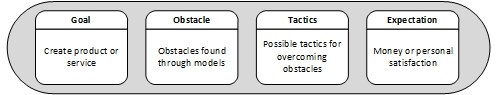
\includegraphics[scale=0.7]{./pics/gote}
\caption{The GOTE method used in entrepreneurship on high level}
\label{fig:gote}
\end{center}
\end{figure}

An interesting take on the GOTE method is the fact that it works on several layers, in both acting and entrepreneurship. This means using the tactics as a new goal, and finding obstacles and tactics for this goal. The expectation for the goal is to come closer to the upper level goal. An example for this in relation to our project can be seen in \figref{fig:gote_watchr}.


\begin{figure}[h]
\begin{center}
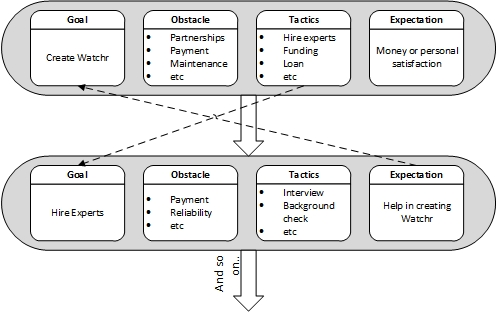
\includegraphics[scale=0.7]{./pics/gote_watchr}
\caption{The GOTE method used several layers for Watchr}
\label{fig:gote_watchr}
\end{center}
\end{figure}

The GOTE method used in entrepreneurship is an ends-driven approach, as it focuses on the goals and expectations. It is linear, as it has little to no possibility in iterations in itself. Apart from these factors, it is possible to use this approach in many aspects, as it is only a tool for process. It is based mainly on concrete situations, and finds the difficulties and obstacles through corporeality. To overcome these difficulties, tactics are found through sociality.